%*********************************************************************
\chapter{CO\textsubscript{2} and Humidity Performance}
\label{ch:co2humidity}
%*********************************************************************

%*********************************************************************
\section{The Gas Connection}
\label{sec:co2c-failure}
%*********************************************************************

The CO\textsubscript{2} loop was to be identified the same way as the thermal loops, by an open loop step test on the built chamber. Pulsing the solenoid at a fixed duty measures the regulator flow $Q_{in}$ and the leak $Q_L$, the two parameters Chapter~\ref{ch:theory} could only estimate, and the decay after the step is a tracer gas decay test in the form of ASTM~E741 \citep{astm_e741}, where the fitted time constant gives $Q_L = V/\tau$. The test code, the pulse schedule and the safety interlocks were written and verified on the hardware. Everything was ready except the gas.

\textbf{The connection leaked.} The regulator's nut screwed smoothly and fully onto the SodaStream adapter, so the joint looked correct. The bottle only arrived the day before the test, so the joint could not be pressure tested any earlier. Opening the cylinder gave a continuous hiss, and soapy water helped find the leak at the adapter to regulator joint. Tightening with two tools did not stop it. The threads were not the cause: the adapter's male thread measured 21.7\,mm, consistent with the W21.8 standard the regulator uses, and the nut was solid when fully tightened. Section~\ref{sec:co2-design} records that the listing's G5/8 claim was wrong and that the supplier confirmed Type 30, so the thread had already been checked once.

\textbf{The seal could not make contact.} The regulator inlet has a filter piece in the middle of its seal, sitting inside the nut (Figure~\ref{fig:co2-leak-photo}). That filter is wider than the opening in the adapter, so it cannot fit inside and it holds the seal off the adapter face. Nothing presses on the seal, so gas passes it. The filter cannot be removed from the regulator. Adding a washer behind the seal pushed it forward far enough to touch, but it also pushed the nut back so only about one thread was still holding. With 57\,bar behind the joint that is not safe, so it was not used.

The regulator would most likely work with a standard CO\textsubscript{2} bottle, so the problem is this adapter. The nut fitted perfectly, so there was no way to find the fault before the bottle arrived and the joint was put under pressure. There are no other SodaStream adapter options and no time left to source a different setup, so the CO\textsubscript{2} loop could not be tested and R4 is not demonstrated on hardware. A regulator with no filter in its inlet, or a normal CO\textsubscript{2} bottle, avoids this.

The rest of this chapter has a different purpose from Chapter~\ref{ch:theory}. There the loop was simulated to check the gains before the hardware existed. Here the geometry is measured, and the two parameters the step test would have given are swept across their plausible range instead, so the next build knows what to measure first and what the design costs if those values are wrong.

%*********************************************************************
\section{The Model for the Built Chamber}
\label{sec:co2-params}
%*********************************************************************
Section~\ref{sec:co2-model} was written before the enclosure was finalised and used the same provisional chamber as the thermal models, $213 \times 155 \times 30$\,mm. The built chamber is smaller and stepped in three sections, and the plate and the two gas sensors take up some of the space inside it. Working through the as-printed geometry gives a free gas volume of 0.47\,L (Table~\ref{tab:co2-volume}), 2.1 times smaller than the 0.99\,L used in Chapter~\ref{ch:theory}. Recomputing from Equation~\ref{eq:co2-tf}, with the leak still taken as two air changes per hour (ACH), gives Table~\ref{tab:co2-gains}.

\begin{table}[htbp]
    \centering
    \caption[CO\textsubscript{2} parameters before and after the volume correction]{\textbf{CO\textsubscript{2} parameters before and after the volume correction.} Gains are per unit duty, with concentration in percentage points.}
    \label{tab:co2-gains}
    \small
    \begin{tabular}{@{}lcc@{}}
        \toprule
         & \textbf{Chapter 3} & \textbf{Corrected} \\
        \midrule
        $V$       & 0.99\,L & 0.47\,L \\
        $Q_L$     & 1.98\,L/h & 0.94\,L/h \\
        $\mu_0$   & 1.72\,\% & 0.82\,\% \\
        $K$       & 273.6\,pp & 576.3\,pp \\
        $\tau$    & 1711\,s & 1711\,s \\
        \midrule
        $K_p$     & 0.0313 & 0.0148 \\
        $K_i$     & $1.83\times10^{-5}$ & $8.68\times10^{-6}$ \\
        \bottomrule
    \end{tabular}
\end{table}

The time constant is unchanged. With the leak written as air changes per hour, $Q_L$ scales with the volume, so $V$ cancels in $\tau = V/(\mu_0 Q_{in} + Q_L)$ and the time constant depends on the exchange rate and not on the size of the chamber. The gain doubles, since the same flow now enters half as much gas, so each unit of duty produces twice the concentration and the controller gains halve. The thermal models in Section~\ref{subsec:sysid-chamber-vs-model} were wrong in the same direction, with the provisional geometry overstating the chamber. $\lambda$ stays at 200\,s. It is a choice about closed loop speed, and correcting the chamber model does not change that choice.

The simulation uses the measured geometry, the full nonlinear balance of Equation~\ref{eq:co2-balance}, and the hardware as built: the solenoid on or off, time proportioned on a 15\,s window with a 0.1\,s minimum pulse, the ExplorIR-M as the 13\,s first order lag of Section~\ref{subsec:co2-control} read twice a second and averaged over 5\,s, and the integral clamped at zero duty. The leak and the flow are swept across their plausible range, since neither was measured.

Three quantities were never measured: the leak, assumed at two air changes per hour; the regulator flow, a design target of 0.1\,L/min never checked on a flow meter; and the mixing delay between the inlet and the sensor, which no sensor in the build can see. CO\textsubscript{2} is denser than air and nothing stirs the 35\,mm deep chamber, so the mixing delay is carried as 0 to 60\,s.

%*********************************************************************
\section{Nominal Performance}
\label{sec:co2-nominal}
%*********************************************************************


The loop fills the chamber to 5\,\% without overshooting. It covers 63.2\,\% of the way in 3.1\,min and settles inside $\pm$0.2\,pp (Figure~\ref{fig:co2-fill}). The valve starts at 7.5\,\% duty and drops to 0.82\,\% once the chamber is at setpoint, so it spends almost all its time shut and has plenty of range left for disturbances. Stability did not change. Halving the volume doubled $K$ and halved the gains, so the loop gain is unchanged and the phase margin is still 83\textdegree{}, or 75\textdegree{} with a 30\,s mixing delay (Figure~\ref{fig:co2-bode}). The fill strategy and the integral freeze from Section~\ref{subsec:co2-control} are unchanged (Figures~\ref{fig:co2-fill-strategies} and~\ref{fig:co2-lid}).

The smaller chamber does change one thing. A single 0.1\,s pulse now adds 0.034\,pp instead of 0.016, and at 0.82\,\% duty the valve needs 0.12\,s per window but can only open in multiples of 0.1\,s (Figure~\ref{fig:co2-pulses}). A 0.1\,s pulse is too little, so the concentration drops a little each window until the valve gives 0.2\,s, which is too much and brings it back up. That rise and fall is 0.078\,pp. That is the smallest ripple this chamber can have, and it is well inside R4.

%*********************************************************************
\section{Sensitivity to the Leak and the Flow}
\label{sec:co2-sensitivity}
%*********************************************************************

The gains depend on two values that were never measured: the leak and the regulator flow. This section covers what the loop does while they stay unknown, and why both need measuring.

Lambda tuning leaves a clean loop, $L(s) = 1/(\lambda s)$, with 90\textdegree{} of phase margin. The real loop is not that. The controller carries the design values $K_m$ and $\tau_m$, the chamber has whatever $K$ and $\tau$ the leak and the flow actually give it, and the sensor and the sampling add lag on top:

\begin{equation}
L(s) = \underbrace{\frac{\tau_m s + 1}{K_m \lambda s}}_{\text{controller}} \cdot
       \underbrace{\frac{K}{\tau s + 1}}_{\text{chamber}} \cdot
       \underbrace{\frac{1}{\tau_s s + 1}}_{\text{sensor}} \cdot
       \underbrace{e^{-\theta s}}_{\text{delays}},
\qquad \theta = \frac{T_s}{2} + \frac{t_{\mathrm{avg}}}{2} + \theta_{\mathrm{mix}}.
\label{eq:co2-loop}
\end{equation}

The leak and the flow were each swept across their plausible range, $K$ and $\tau$ recomputed at every point, and the phase margin taken from Equation~\ref{eq:co2-loop} with a 60\,s mixing delay assumed. Figure~\ref{fig:co2-sweeps} shows both sweeps, and Figure~\ref{fig:co2-robustness} shows the fill itself at the ends of each range.

\textbf{A wrong leak costs speed, not stability.} From Equation~\ref{eq:co2-tf}, the leak sits in the denominator of both $K$ and $\tau$, so it shrinks them together and the margin barely moves. The fill is what suffers. The controller carries a 29\,min time constant, while a chamber at twelve air changes per hour settles in 4.8\,min and needs six times the duty to hold 5\,\%. That duty has to come from the integral, which still builds at the rate set for 29\,min, so the chamber reaches 4\,\% quickly and then crawls, reaching only 4.77\,\% after 90 minutes. The ripple grows with it, from 0.078\,pp to 0.30\,pp, since each valve opening has to be longer.

\textbf{A wrong flow costs stability.} A faster flow leaves the chamber no fuller, since the valve opens for less time, so $\tau$ is unchanged and the whole error lands on $K$. A larger $K$ pushes the crossover higher, where the delay $\theta$ costs much more phase. The margin falls from 78\textdegree{} at 0.05\,L/min to 20\textdegree{} at 0.3\,L/min.

\begin{figure}[htbp]
    \centering
    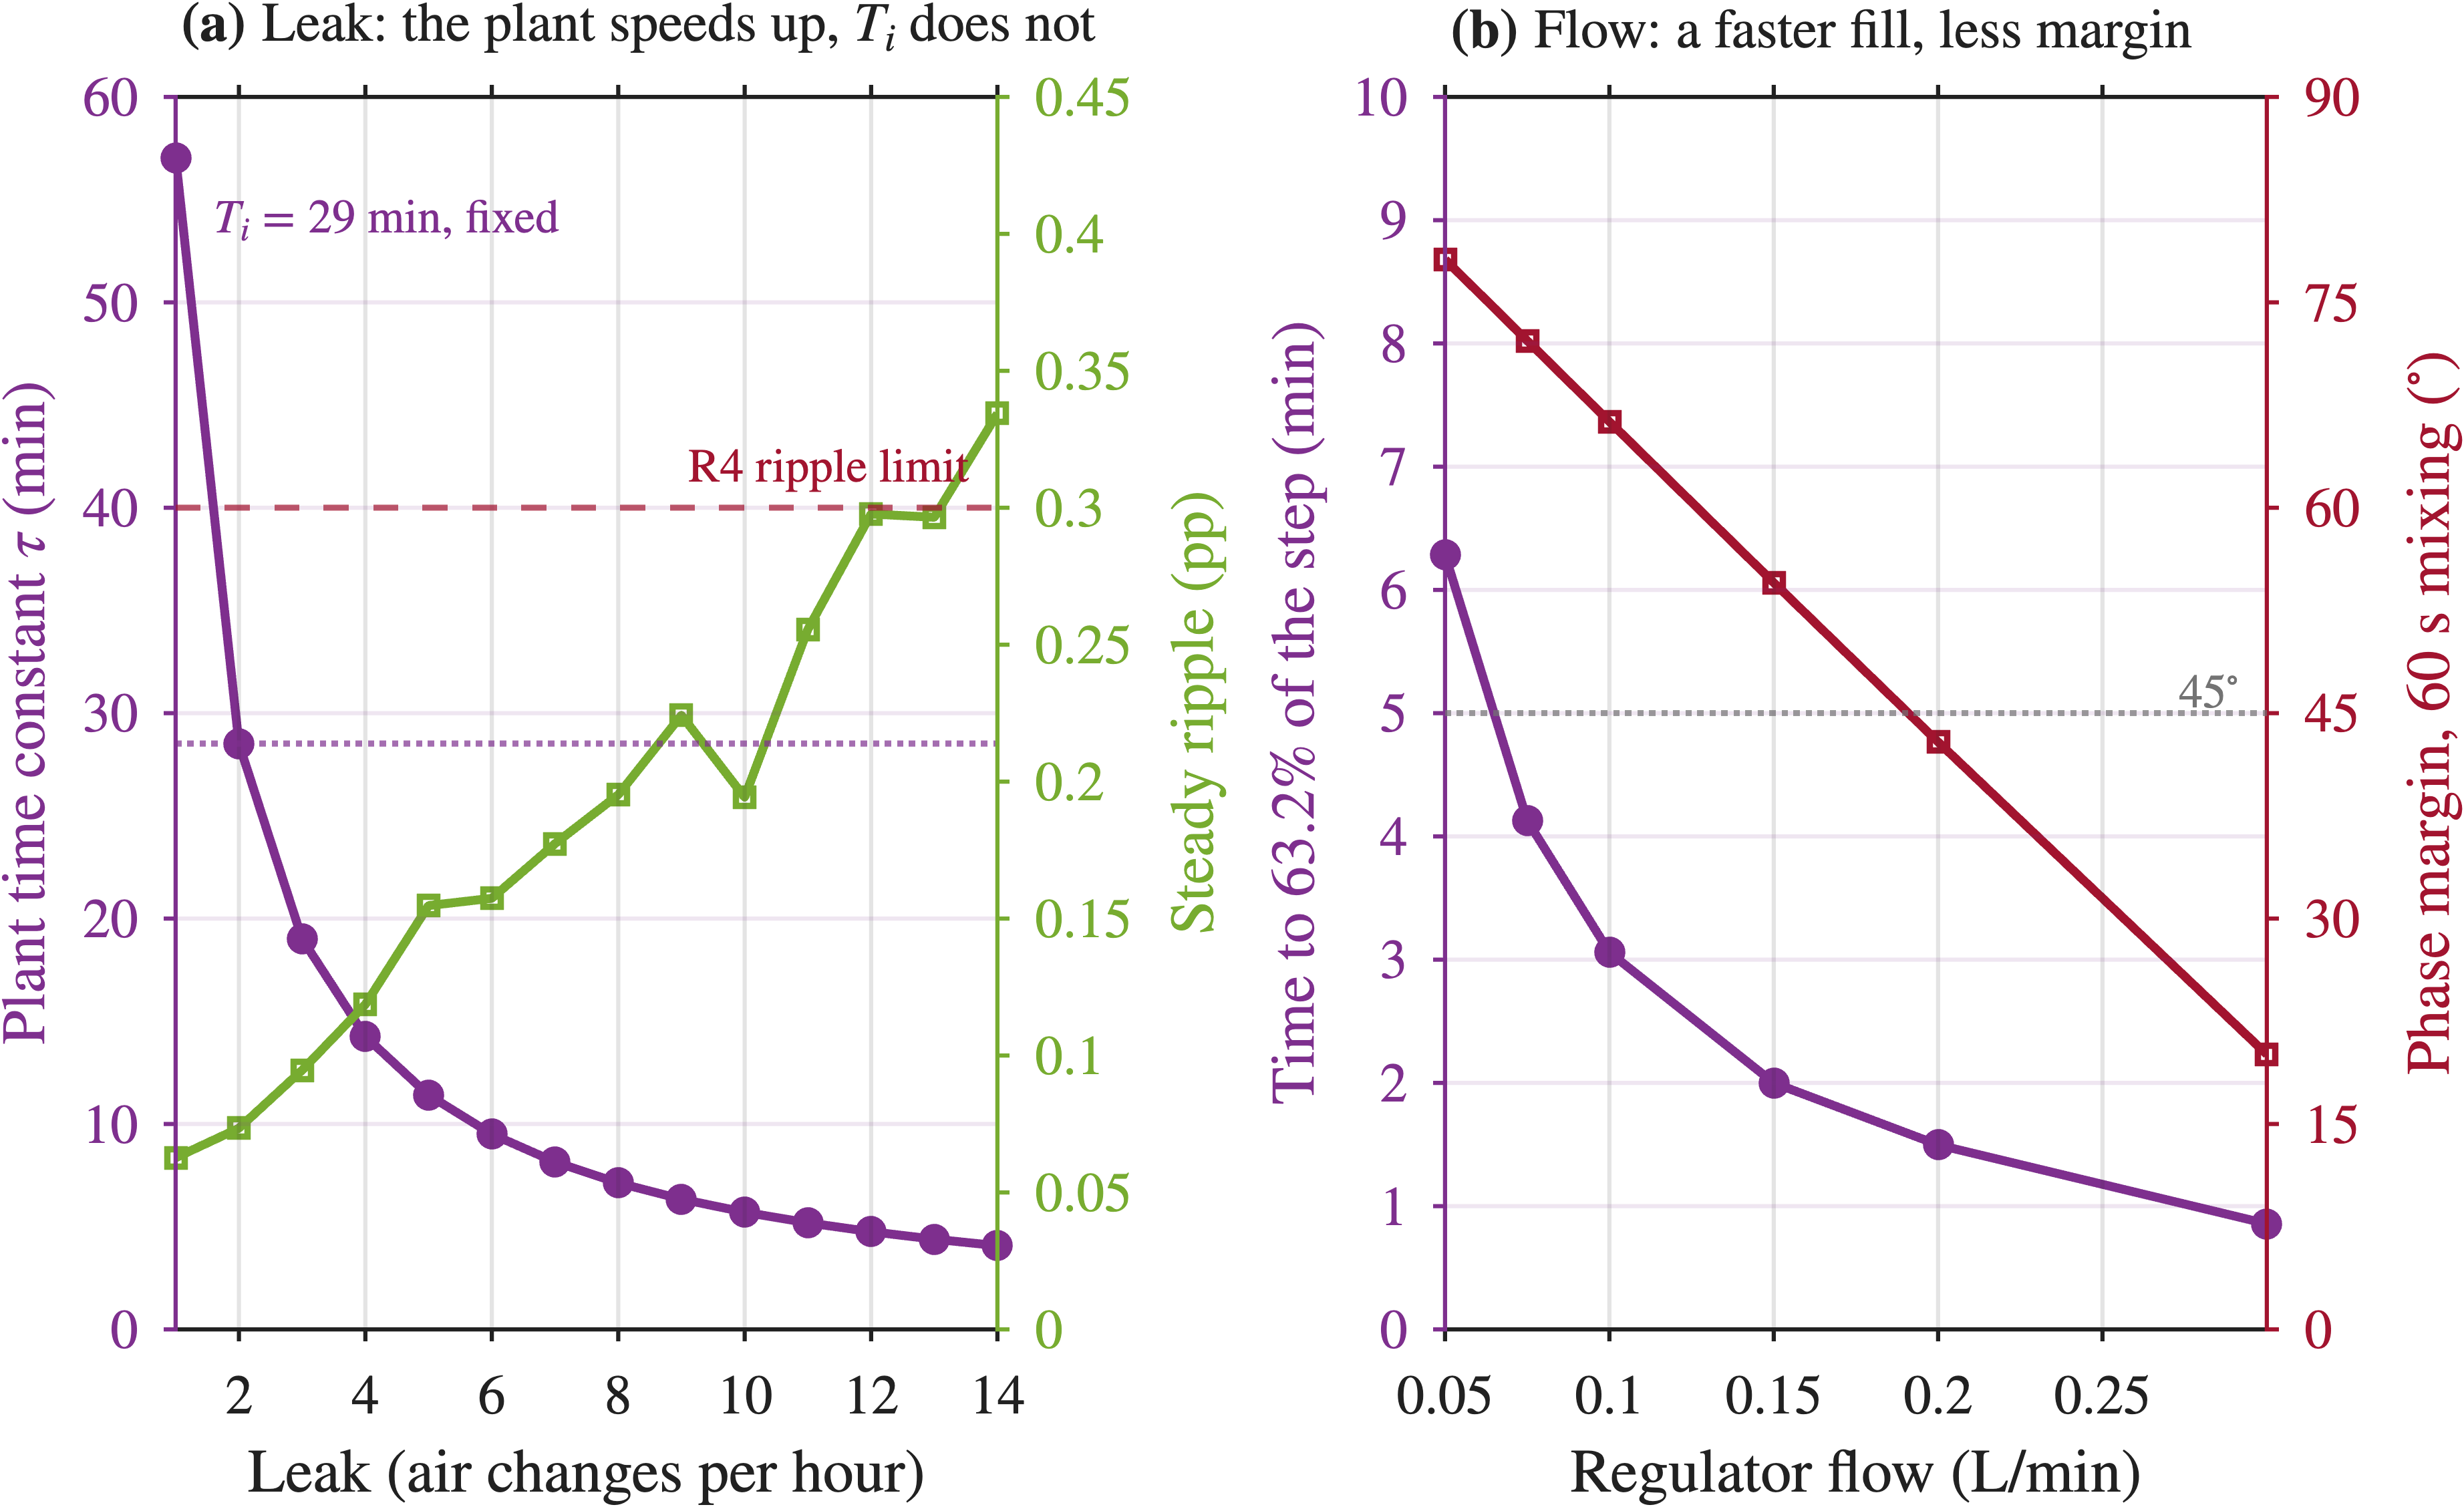
\includegraphics[width=0.95\textwidth]{figs/ch8/NEW_fig_C8_sweeps.png}
    \caption[Sensitivity to the leak and the flow]{\textbf{Sensitivity to the two unmeasured parameters.} Each panel carries two quantities on separate axes, coloured to match. (a) Solid purple: the chamber's actual time constant, falling as the leak rises. Dotted purple: the time constant the controller assumes, fixed at 29\,min by the gains. Green: the height of the sawtooth. Dashed red: 0.3\,pp, half of R4's 0.6\,pp band, taken as the budget for ripple alone. (b) Purple: time to reach 63.2\,\% of the fill. Red: phase margin with a 60\,s mixing delay assumed. Dotted grey: 45\textdegree{} phase margin.}
    \label{fig:co2-sweeps}
\end{figure}

In panel (a) the two purple lines meet only at two air changes per hour, and everything to the right of that is the controller working against a chamber it does not match. The green curve reaches the ripple budget at twelve. In panel (b) a faster fill costs margin, and the margin passes 45\textdegree{} at about twice the design flow. A wrong leak costs fill time and ripple. A wrong flow costs stability margin. Neither needs the controller restructured, and both go away once the value is measured and the gains are recomputed from Equation~\ref{eq:lambda-gains}.

Four things follow for the first run on gas. \textbf{Set the needle valve at or below 0.1\,L/min}, since halving the flow costs about ten minutes on a fill at the start of an experiment, and keeps 75\textdegree{} of phase margin even if mixing is slow. \textbf{Measure the leak first}, as it is the dominant unknown: the decay phase already written into the step test gives $Q_L = V/\tau$ from a single exponential fit and needs only a working CO\textsubscript{2} sensor and a sealed chamber, after which the gains follow from Equation~\ref{eq:lambda-gains}. \textbf{Seal the gland and the gas line}, since Section~\ref{sec:sysid-approach} records both as open during the thermal step tests and an unsealed chamber is the one condition under which two air changes per hour is optimistic. \textbf{Lengthen the control period if the measured leak is high}, because the sawtooth grows with the leak and reaches the 0.3\,pp budget at about twelve air changes per hour, and a 30\,s window halves the duty resolution to 0.33\,\% at $T_s/\lambda = 0.15$, still well inside the sampling limit.

R4 is not demonstrated. The loop is designed and the simulation meets R4 across a wide range of the unmeasured parameters, but it could not be tested on gas.

%*********************************************************************
\section{Humidity}
\label{sec:humidity}
%*********************************************************************

The chamber was to be humidified by passing the incoming CO\textsubscript{2} through a water reservoir (Section~\ref{sec:co2-design}), so the gas arrived wet. That path runs through the gas connection, which never worked, so it was never tested.

\textbf{The humidified gas line would not have humidified the chamber enough.} The chamber is not sealed, so it exchanges air with the room continuously. The supply is pure CO\textsubscript{2} and the chamber only needs 5\,\%, so very little gas has to go in to hold it there, and only about a twentieth of the air entering comes through the regulator. The rest leaks in from the room. That fraction is set by the two concentrations and holds whatever the leak rate turns out to be. A humidified gas line would therefore wet a twentieth of the incoming air and leave the rest at room humidity. What the design needs is a separate vessel holding 5\,\% CO\textsubscript{2} in air, pumped continuously through heated water, so the flow is set by a pump and not by the control valve. That is a different architecture and belongs in the next iteration.

\textbf{What the build can do instead is passive.} Water is placed in the wells of the plate and evaporates into the chamber air, which the heaters keep warm. Nothing controls it. The plate is the wrong place for the water, since in a real experiment the wells hold the sample and evaporation out of them is what humidification exists to prevent. No cells are grown here, so the plate serves as a convenient reservoir to answer a narrower question: with water at chamber temperature, what humidity does this chamber reach.

\textbf{The sensing available for the run.} Two of the four thermistors failed during testing, both at the leads, which are thin and unsupported where they leave the probe: the corner probe and the probe on the lid glass. The room thermistor was moved onto the glass so that the glass loop could keep running, and the room temperature was then taken from a BMP280 outside the chamber. The BMP280 is a pressure and temperature sensor read over the existing I\textsuperscript{2}C bus, accurate to $\pm$1\,\textdegree{}C between 0 and 65\,\textdegree{}C \citep{bosch_bmp280}, which is adequate for a disturbance input that is not used for control. The SCD30 stopped responding partway through an earlier test and was not recovered. Humidity was measured instead with a DHT22 under the lid, specified to $\pm$2\,\% RH and $\pm$0.5\,\textdegree{}C at a resolution of 0.1 \citep{aosong_dht22}. It uses a single-wire protocol, read every 2\,s with a checksum on each frame and up to three retries before a reading is logged as missing. The DHT22 also reports its own temperature, so the reading can be corrected to the chamber air temperature from the PT1000.

\textbf{The run.} The chamber was held at 39\,\textdegree{}C and the lid glass at 44\,\textdegree{}C with the base heater out of circuit, logging every channel at 5\,s. The run was planned to last 24 hours, so that R8 could be tested at the same time, and reached 6\,h\,33\,min before a connection failed. A CO\textsubscript{2} incubator normally runs at 90 to 95\,\% relative humidity, which is what R3 asks for and what the measurement is compared against.

\begin{figure}[htbp]
    \centering
    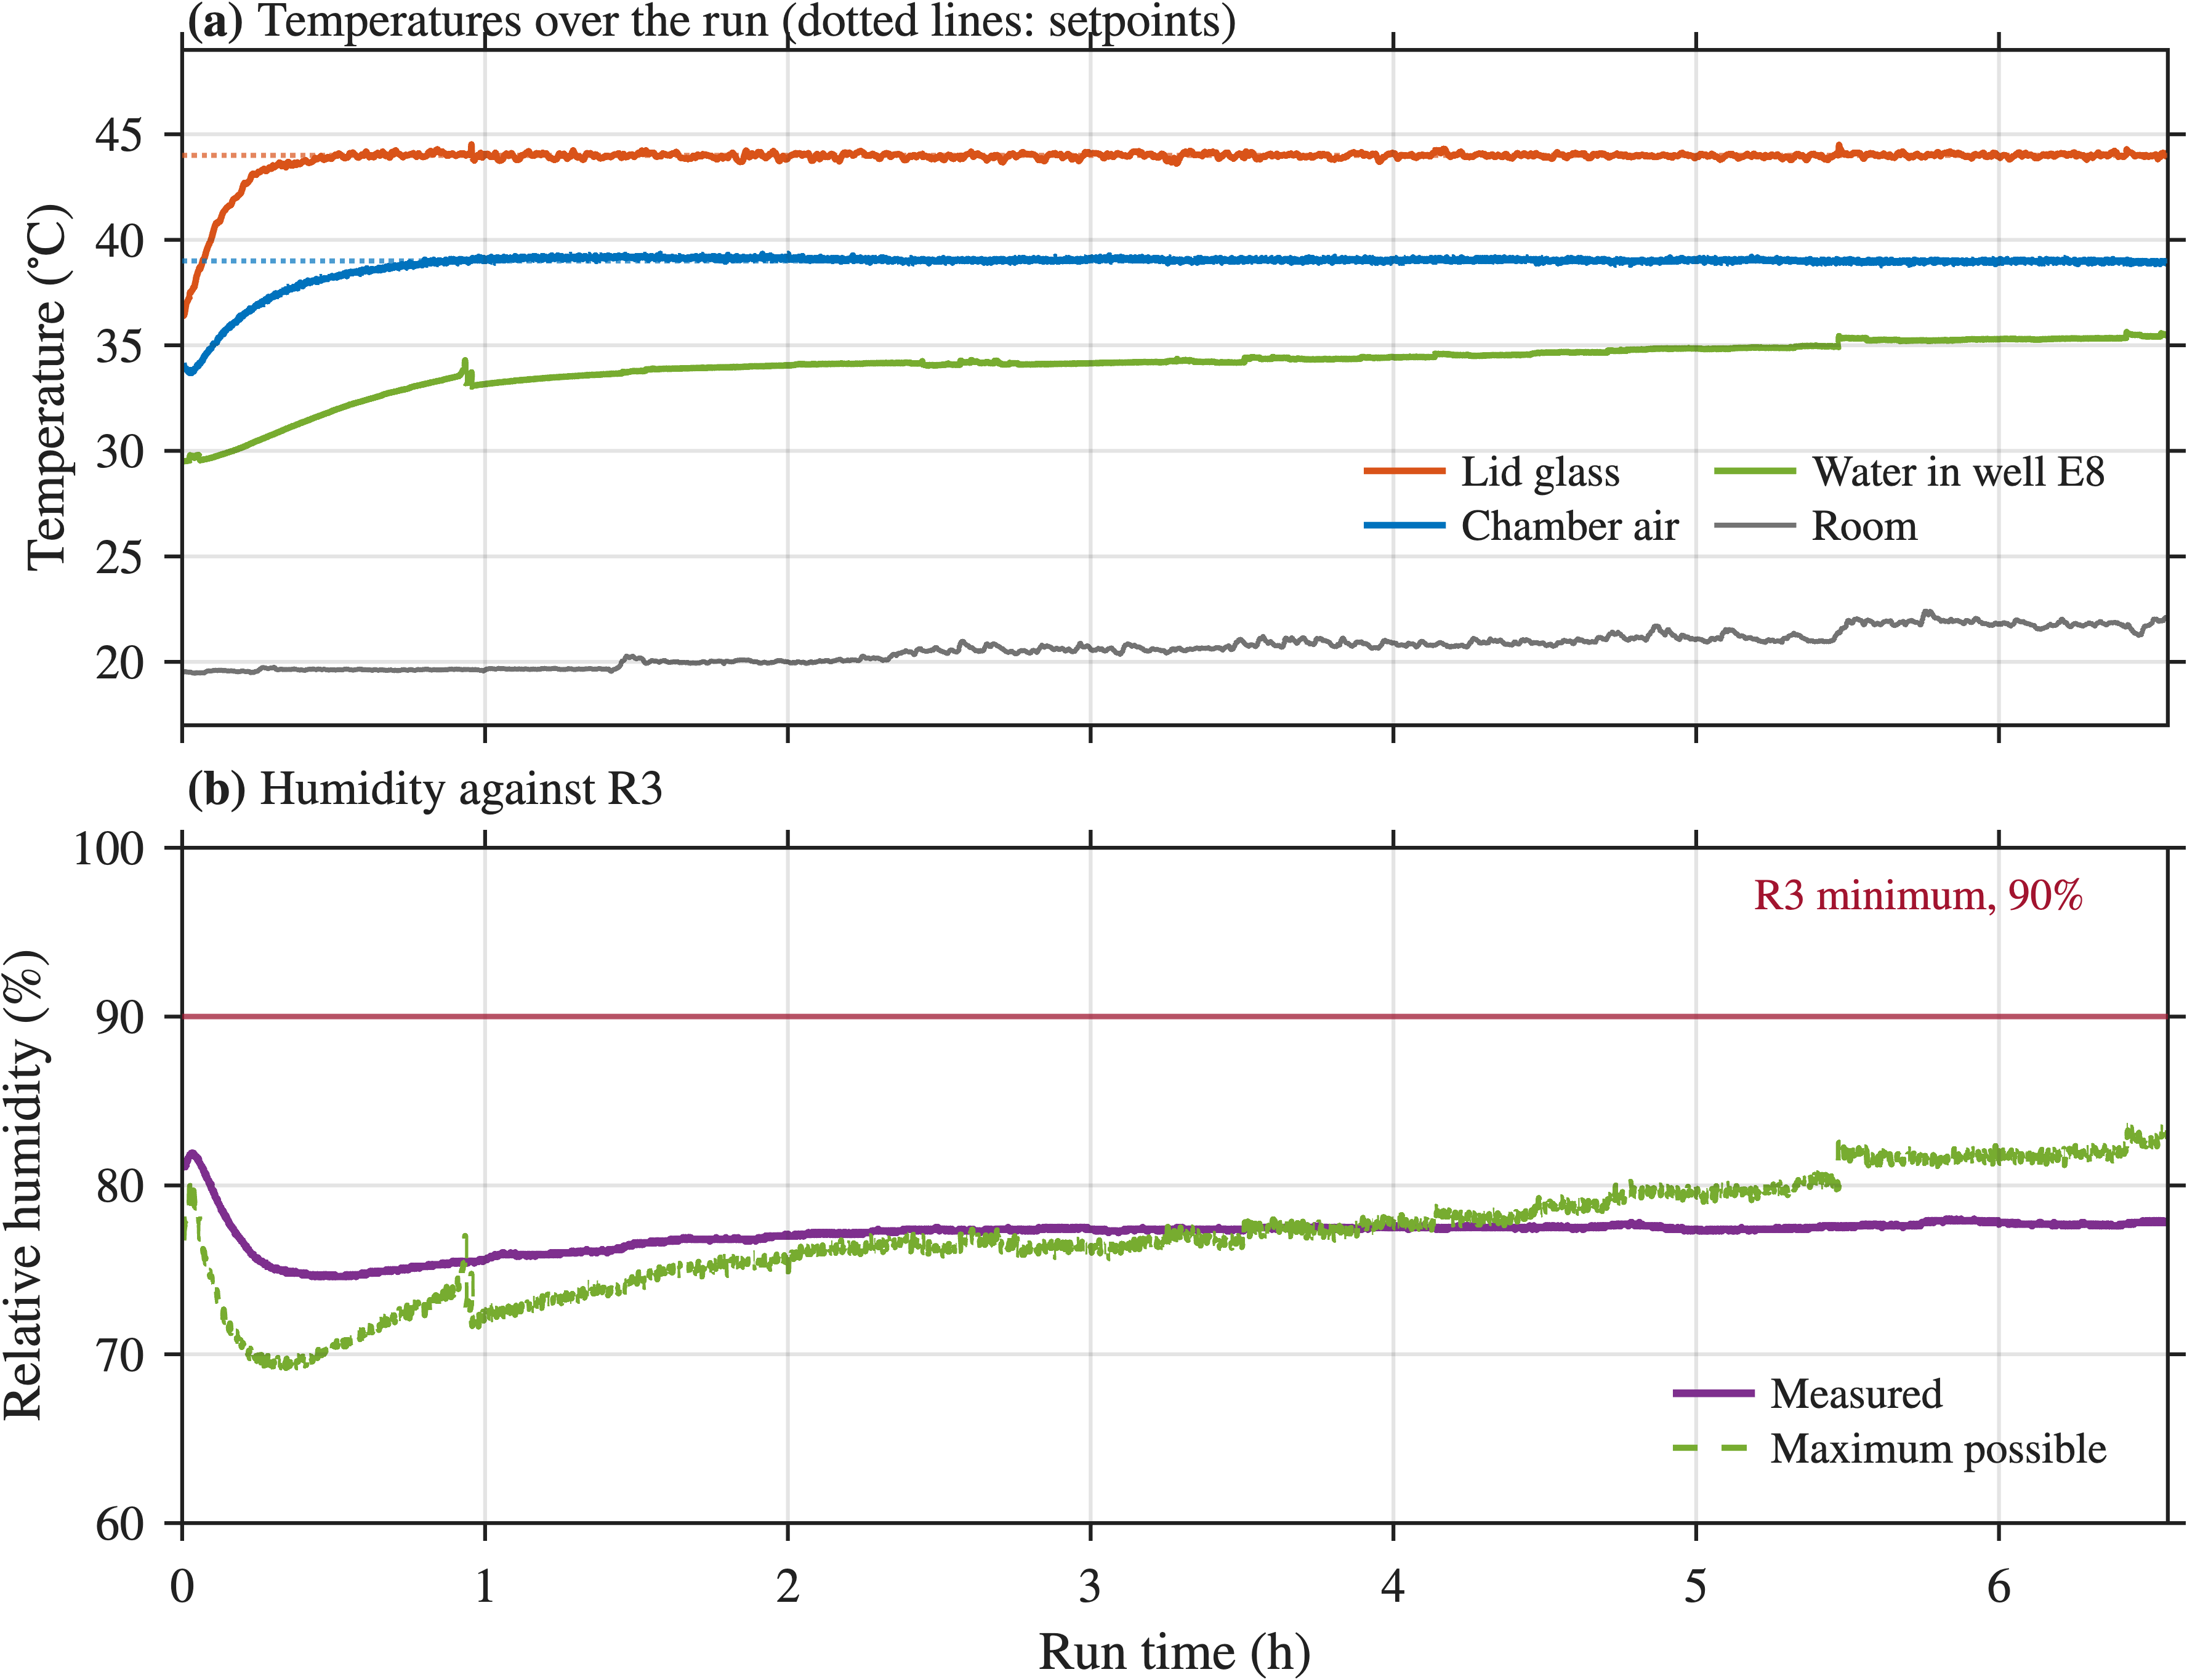
\includegraphics[width=0.8\textwidth]{figs/ch8/fig_H1_long_run.png}
    \caption[The long run]{\textbf{The long run.} (a) All four temperatures, with the setpoints dotted. (b) Measured humidity against R3. The dashed green line is the highest humidity possible at each moment, calculated from Equation~\ref{eq:rh-ceiling} using the measured water and air temperatures.}
    \label{fig:humid-run}
\end{figure}

\textbf{Both loops held for the whole run.} Table~\ref{tab:humid-steady} gives the steady values over the 5.6\,h after warm-up. The chamber held 39.045\,\textdegree{}C with a standard deviation of 0.074\,\textdegree{}C and the glass 43.99\,\textdegree{}C, through a room that rose from 19.6 to 22.4\,\textdegree{}C. That is a disturbance nearly three times larger than the 1\,\textdegree{}C of room drift in Section~\ref{sec:cl-test1}, and neither loop moved off setpoint. The PT1000 returned no fault on any of the 5015 logged rows. The glass stayed 9.5\,\textdegree{}C above the dew point throughout, so R5 held on the optical path with a wide margin.

\begin{table}[htbp]
    \centering
    \caption[Steady values over the long run]{\textbf{Steady values over the long run,} averaged across the 5.6\,h after warm-up.}
    \label{tab:humid-steady}
    \small
    \begin{tabular}{@{}lcc@{}}
        \toprule
        & \textbf{Mean} & \textbf{Std dev} \\
        \midrule
        Chamber air (\textdegree{}C)      & 39.045 & 0.074 \\
        Lid glass (\textdegree{}C)        & 43.992 & 0.096 \\
        Water in well E8 (\textdegree{}C) & 34.471 & 0.554 \\
        Room (\textdegree{}C)             & 20.819 & 0.673 \\
        Relative humidity (\%)            & 77.30  & 0.48 \\
        Dew point (\textdegree{}C)        & 34.48  & 0.13 \\
        \midrule
        Heater duty (\%)                  & 64.0 & 2.3 \\
        Glass duty (\%)                   & 73.5 & 2.9 \\
        \bottomrule
    \end{tabular}
\end{table}

\textbf{R3 is not met.} The humidity settled at a mean of 77.3\,\% (Table~\ref{tab:humid-steady}) and stayed there for hours, against the 90\,\% minimum R3 asks for. The cause is the water sitting colder than the air. Relative humidity is how much of the air's water capacity is used, and that capacity, $p_{sat}$, depends only on temperature. Air sitting over the water becomes saturated at the water's temperature, and the heaters then warm that air to the chamber setpoint, raising the capacity but not the water it carries:

\begin{equation}
\mathrm{RH}_{\max} = \frac{p_{sat}(T_{water})}{p_{sat}(T_{air})},
\label{eq:rh-ceiling}
\end{equation}

with $p_{sat}$ from the Magnus relation, $p_{sat}(T) = 6.1094\exp\!\left(17.625T/(243.04+T)\right)$\,hPa \citep{alduchov_improved_1996}.

The gap between the water and the air therefore sets the highest humidity the chamber can reach, and near 39\,\textdegree{}C each degree of gap costs about five percentage points. Holding 90\,\% with the air at 39\,\textdegree{}C needs the water at 37.0\,\textdegree{}C, a gap of 2.0\,\textdegree{}C. The water sat at 34.5\,\textdegree{}C, a gap of 4.6\,\textdegree{}C, so $p_{sat}$ is 54.6 against 69.9\,hPa and the ceiling is 78\,\%, matching the 77.3\,\% measured. The dashed line in Figure~\ref{fig:humid-run}b is that ceiling evaluated through the run, rising as the water warms. More water in more wells changes nothing, since the limit is the gap and not the amount of water. For about the first two hours the measurement sits above that line, by up to about 5 percentage points early in the warm-up. This lies within the uncertainty of the comparison: the DHT22 is specified to $\pm$2\,\% RH, and up to $\pm$5\,\% at the extremes of its range \citep{aosong_dht22}, and the well probe rests on the floor of one well, so it reads the coldest water in the plate while the evaporating surface is likely warmer, which places the true ceiling higher. Late in the run the measurement falls slightly below the line, since the small evaporating area in the wells cannot keep up with what the leak removes.

\begin{figure}[!htbp]
    \centering
    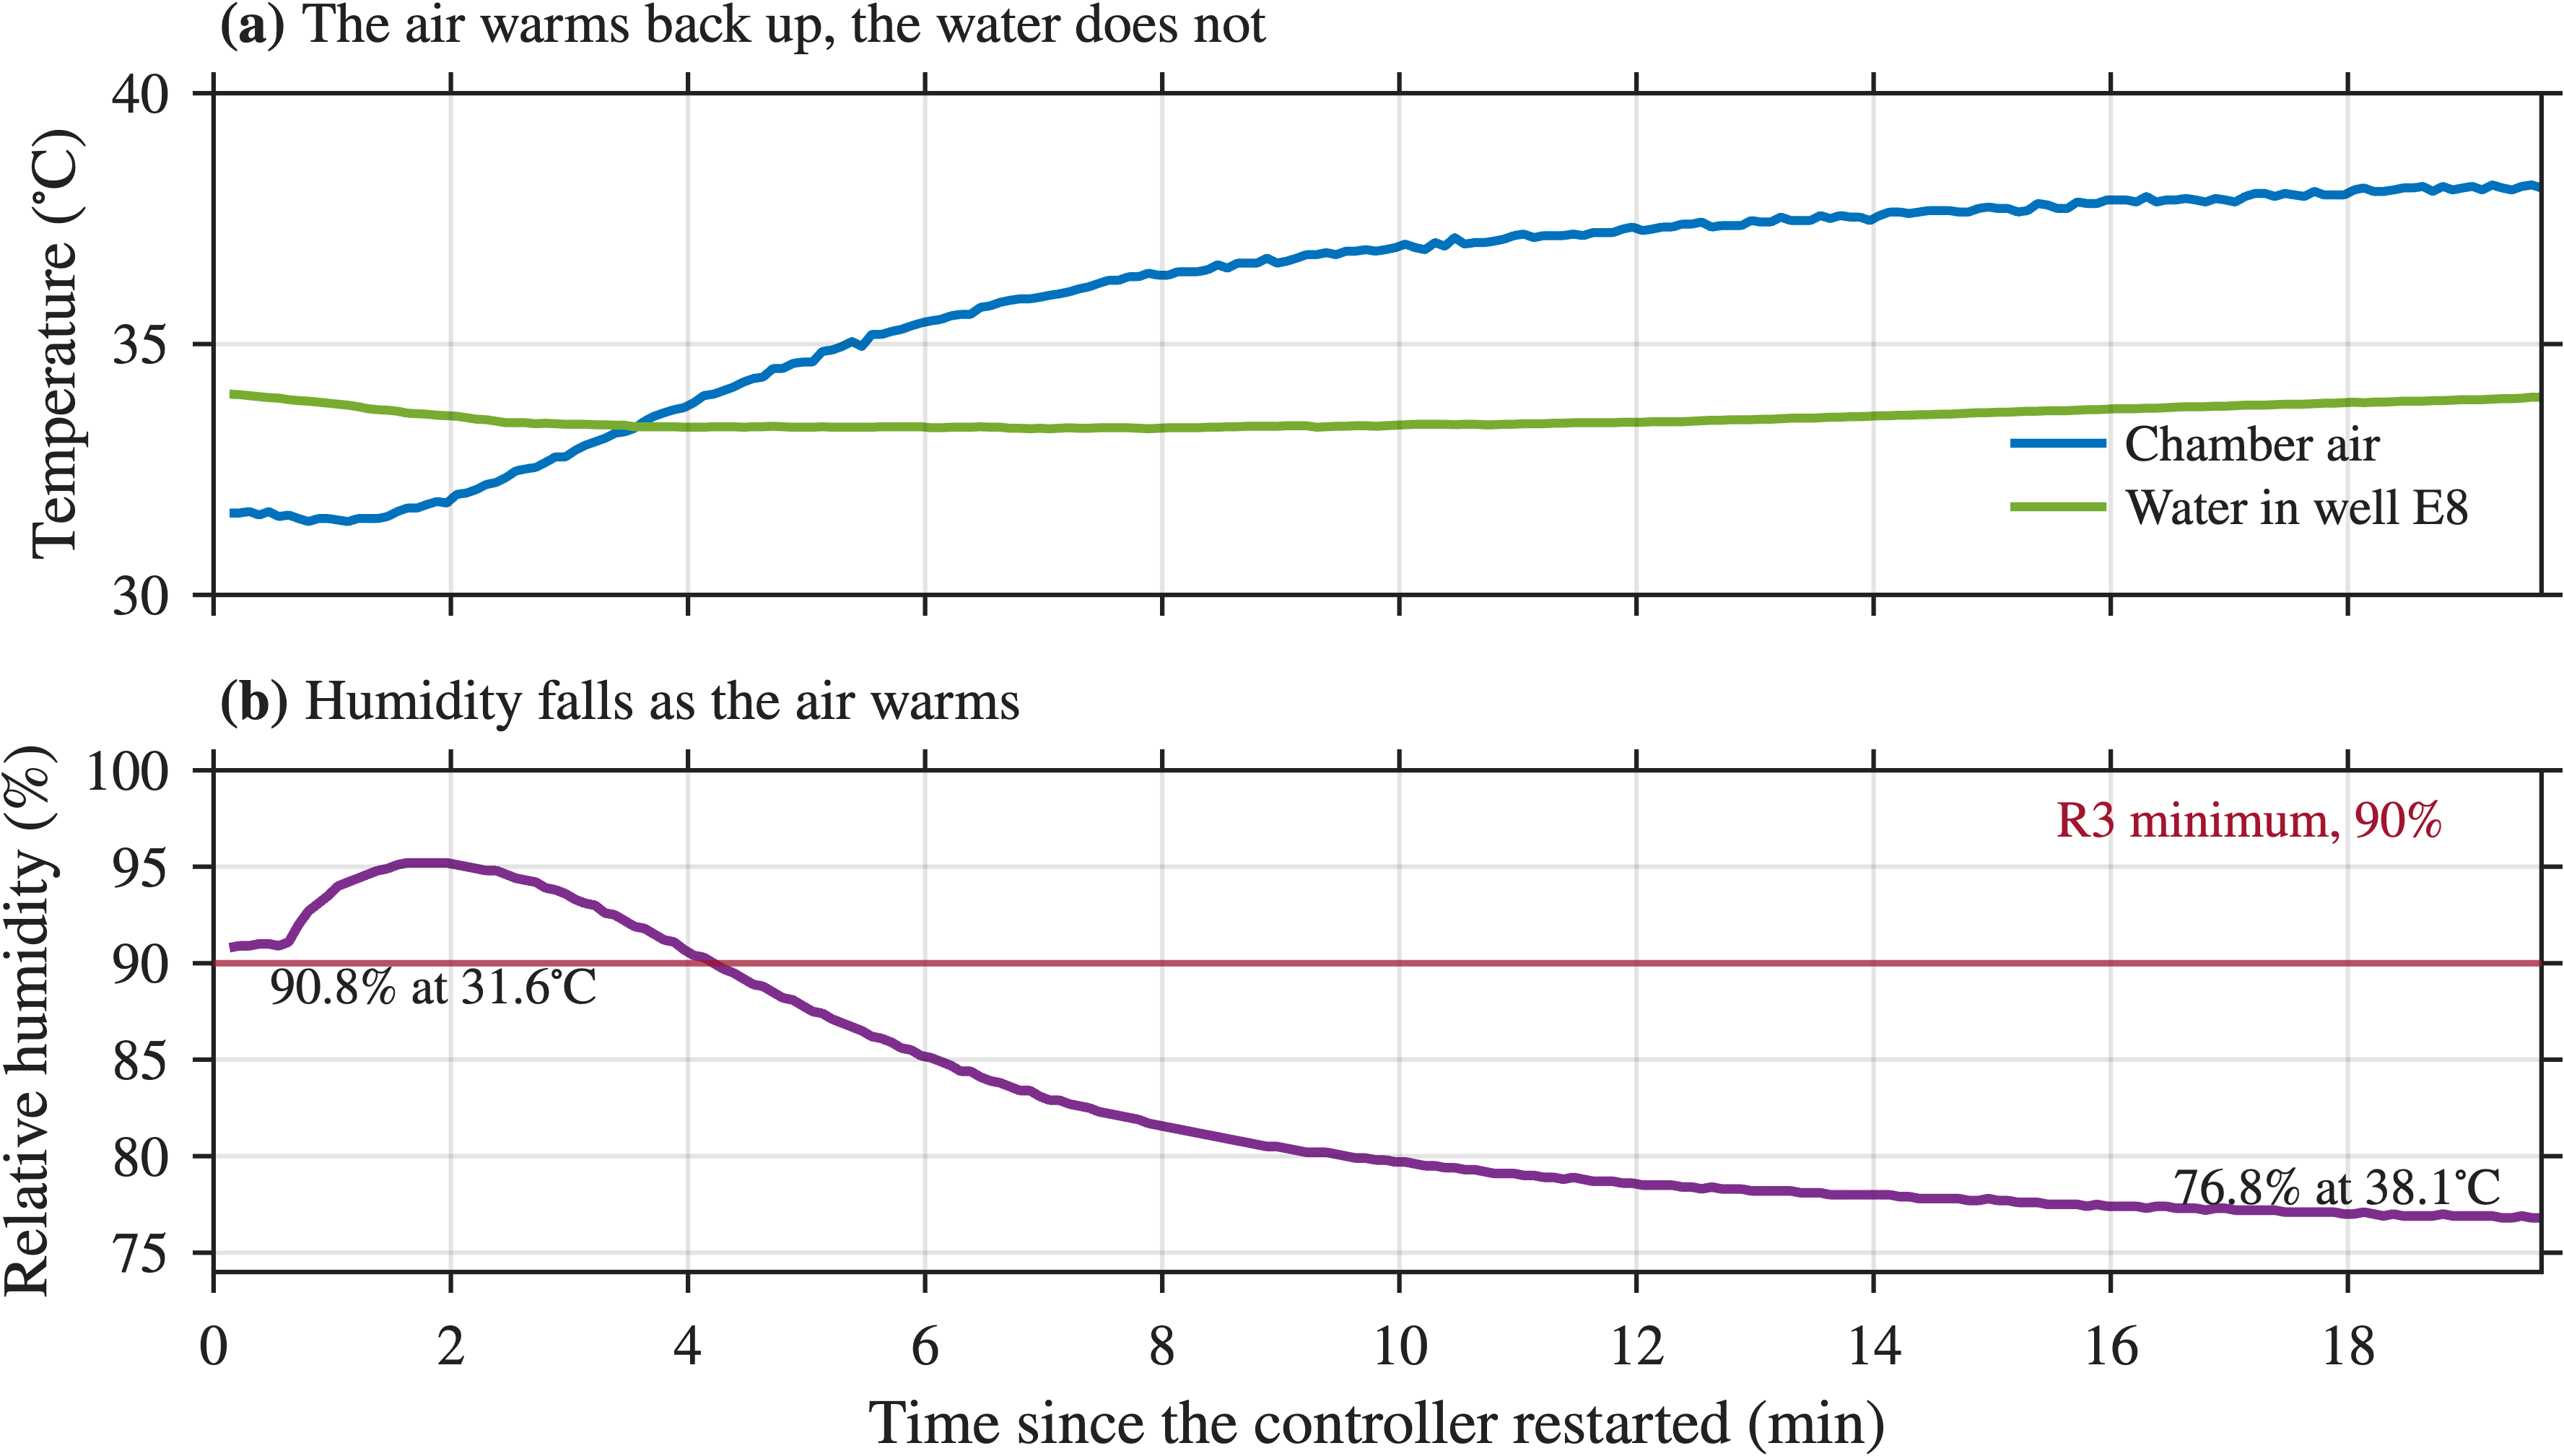
\includegraphics[width=0.8\textwidth]{figs/ch8/fig_H3_restart.png}
    \caption[The restart after the fault]{\textbf{The restart after the fault.} (a) The heaters bring the air back up while the water in the wells stays where it is. (b) The humidity falls as the gap between the water and the air opens again.}
    \label{fig:humid-restart}
\end{figure}

\textbf{The reset showed the effect both ways.} When the controller reset the heaters went off for ten minutes. The air fell to 31.6\,\textdegree{}C while the water stayed at 34.0\,\textdegree{}C, so the water was now warmer than the air, and the humidity read 90.8\,\%. Over the next twenty minutes the heaters brought the air back to 38.1\,\textdegree{}C with the water unchanged, and the humidity fell to 76.8\,\% (Figure~\ref{fig:humid-restart}). The same chamber and the same water give 78\,\% with the water 4.5\,\textdegree{}C below the air and 91\,\% with it 2.4\,\textdegree{}C above.

\textbf{Condensation formed where the chamber is coldest.} Droplets appeared in the corners of the enclosure during the run, without pooling. The corner probe was one of the two thermistors lost before this run, but Section~\ref{sec:cl-test1} puts the corner at 0.424 of the climb from room to chamber air, placing it near 28.5\,\textdegree{}C here, about 6\,\textdegree{}C below the dew point. Condensation there follows. The glass fogged within minutes of the heaters going off at the reset and stayed clear whenever they were running, which confirms that the glass heater is what keeps the optical path clear.

Condensation inside the enclosure still matters for longer runs. Water collecting on cold walls is water removed from the air, and liquid anywhere in the enclosure is a contamination route in the BSL-3 setting this is intended for. Keeping the whole enclosure above the dew point means heating or insulating the corners, where the wall penetrations carry heat away (Section~\ref{sec:cl-test1}).

\textbf{The base heater raises the humidity as well as the sample.} Reaching 90\,\% at 39\,\textdegree{}C air needs the water at 37.0\,\textdegree{}C, 2.0\,\textdegree{}C below the air instead of 4.6. The water sits at the sample temperature, and Section~\ref{sec:cl-test3} showed heating from below lifts that from 30.9 to 36.7\,\textdegree{}C with the air unchanged. One change addresses R2 and R3 together, and it also speeds up evaporation, which is what held the chamber below the ceiling late in this run. The base was out of circuit here, so this is a prediction and not a measurement. Chapter~\ref{ch:furtherwork} names the test that would confirm it.

\textbf{R8 is not met.} The run was intended to last 24 hours and reached 6\,h\,33\,min, ending when an I\textsuperscript{2}C connection worked loose and reset the controller. The rig is wired with jumper leads throughout and had been moved several times during testing, and three other connections had already failed: the two thermistor leads, one of them on the glass, and the SCD30. No time remained to rebuild the wiring. Across the whole run no loop tripped and the PT1000 fault code stayed clear, so the failures are in the interconnect and not in the control or the sensing. Chapter~\ref{ch:furtherwork} takes this as the case for a printed circuit board with proper terminations before an unattended run of this length is attempted again.

\textbf{Passive humidification is not the answer regardless.} Standing water inside the chamber cannot be controlled or adjusted during a run and is not acceptable for the BSL-3 work this incubator is ultimately intended for. The result argues for an active supply in the next design.